\documentclass[tikz]{standalone}
\usetikzlibrary{datavisualization}
\usetikzlibrary{datavisualization.formats.functions}
\begin{document}
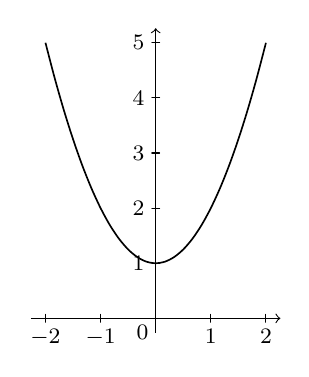
\begin{tikzpicture}[scale=.7]
	\datavisualization [school book axes, visualize as smooth line]
	data [format=function] {
	  var x : interval [-2:2];
	  func y = \value x*\value x + 1;
	};
\end{tikzpicture}

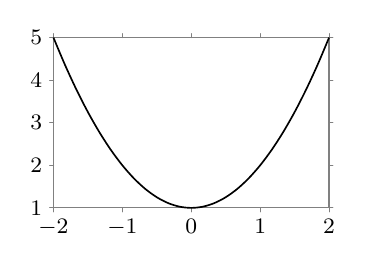
\begin{tikzpicture}[scale=.7]
  \datavisualization [scientific axes, visualize as smooth line]
  data [format=function] {
	var x : interval [-2:2];
	func y = \value x*\value x + 1;
  };
\end{tikzpicture}

\end{document}
